%!TEX encoding = UTF-8 Unicode
%!TEX root = ../lect-w01.tex

%%%%%%%%%%%%%%%%%%%%%%%%%%%%%%%%%%%%%%
\Subsection{Om kursen}

%%%

\ifkompendium
\begin{Slide}{Veckoöversikt}
\noindent\resizebox{0.9\columnwidth}{!}{
%!TEX encoding = UTF-8 Unicode
\begin{tabular}{l|l|l|l}
\textit{W} & \textit{Modul} & \textit{Övn} & \textit{Lab} \\ \hline \hline
W01 & Introduktion            & expressions & kojo            \\
W02 & Kodstrukturer           & programs    & --              \\
W03 & Funktioner, Objekt      & functions   & bugs            \\
W04 & Datastrukturer          & data        & pirates         \\
W05 & Sekvensalgoritmer       & sequences   & cards           \\
W06 & Klasser, Likhet         & classes     & turtlegraphics  \\
W07 & Arv, Gränssnitt         & traits      & turtlerace-team \\
KS  & KONTROLLSKRIVN.         & --          & --              \\
W08 & Mönster, Undantag       & matching    & chords-team     \\
W09 & Matriser, Typparametrar & matrices    & maze            \\
W10 & Sökning, Sortering      & sorting     & surveydata-team \\
W11 & Scala och Java          & scalajava   & lthopoly-team   \\
W12 & Trådar                  & threads     & life            \\
W13 & Design                  & Uppsamling  & Projekt         \\
W14 & Tentaträning            & Extenta     & --              \\
T   & TENTAMEN                & --          & --              \\
\end{tabular}

}
\end{Slide}


\noindent Kursen består av en \textbf{modul} per läsvecka med två \textbf{föreläsningar}, en \textbf{övning} och en \textbf{laboration} (undantaget W02, W13 \& W14 som saknar labb och/eller övning).
Föreläsningarna ger en översikt av den teori som ingår i varje modul. Genom att göra övningarna bearbetar du teorin och förebereder dig inför laborationerna. När du klarat övningen och laborationen i en modul är du redo att gå vidare till nästa. Tabellen på nästa uppslag visar begrepp som ingår i varje modul.

Kursen är uppdelad i två läsperioder. Efter första läsperioden gör du en diagnostisk \textbf{kontrollskrivning} som kontrollerar ditt kunskapsläge. Andra läsperioden avslutas med ett större \textbf{projekt} och en skriftlig \textbf{tentamen}.

\clearpage
\hyphenation{intro-duktion sekvens-algoritmer kod-strukturer data-strukturer}
{%\fontsize{11}{13}\selectfont
\renewcommand{\arraystretch}{1.75}
\begin{longtable}{@{}p{.05\textwidth} | >{\hspace{0.1em}\raggedright\bfseries\sffamily}p{.15\textwidth}  >{\raggedleft\arraybackslash\hspace{0.0em}%\fontsize{10.5}{12}\selectfont
}p{0.735\textwidth}}
W01 & Introduktion & sekvens, alternativ, repetition, abstraktion, programmeringsspråk, programmeringsparadigmer, editera-kompilera-exekvera, datorns delar, virtuell maskin, REPL, literal, värde, uttryck, identifierare, variabel, typ, tilldelning, namn, val, var, def, inbyggda typer, Int, Long, Short, Double, Float, Byte, Char, String, println, typen Unit, enhetsvärdet (), stränginterpolatorn s, if, else, true, false, MinValue, MaxValue, aritmetik, slumptal, math.random, logiska uttryck, de Morgans lagar, while-sats, for-sats \\
W02 & Kodstrukturer & iterering, for-uttryck, map, foreach, Range, Array, Vector, algoritm vs implementation, pseudokod, algoritm: SWAP, algoritm: SUM, algoritm: MIN/MAX, algoritm: MININDEX, block, namnsynlighet, namnöverskuggning, lokala variabler, paket, import, filstruktur, jar, dokumentation, programlayout, JDK, main i Java vs Scala, java.lang.System.out.println \\
W03 & Funktioner, objekt & definera funktion, anropa funktion, parameter, returtyp, värdeandrop, namnanrop, default-argument, namngivna argument, applicera funktion på alla element i en samling, procedur, värdeanrop vs namnanrop, uppdelad parameterlista, skapa egen kontrollstruktur, objekt, modul, punktnotation, tillstånd, metod, medlem, funktionsvärde, funktionstyp, äkta funktion, stegad funktion, apply, lazy val, lokala funktioner, anonyma funktioner, lambda, aktiveringspost, anropsstacken, objektheapen, rekursion  cslib.window.SimpleWindow \\
W04 & Datastrukturer & attribut (fält), medlem, metod, tupel, klass, Any, isInstanceOf, toString, case-klass, samling, scala.collection, föränderlighet vs oföränderlighet, List, Vector, Set, Map, typparameter, generisk samling som parameter, översikt samlingsmetoder, översikt strängmetoder, läsa/skriva textfiler, Source.fromFile, java.nio.file \\
W05 & Sekvensalgoritmer & sekvensalgoritm, algoritm: SEQ-COPY, in-place vs copy, algoritm: SEQ-REVERSE, algoritm: SEQ-REGISTER, sekvenser i Java vs Scala, for-sats i Java, java.util.Scanner, scala.collection.mutable.ArrayBuffer, StringBuilder, java.util.Random, slumptalsfrö \\
W06 & Klasser & objektorientering, klass, Point, Square, Complex, new, null, this, inkapsling, accessregler, private, private[this], kompanjonsobjekt, getters och setters, klassparameter, primär konstruktor, objektfabriksmetod, överlagring av metoder, referenslikhet vs strukturlikhet, eq vs == \\
W07 & Arv & arv, polymorfism, trait, extends, asInstanceOf, with, inmixning, supertyp, subtyp, bastyp, override, klasshierarkin i Scala: Any AnyRef Object AnyVal Null Nothing, referenstyper vs värdetyper, klasshierarkin i scala.collection, Shape som bastyp till Point och Rectangle, accessregler vid arv, protected, final, klass vs trait, abstract class, case-object, typer med uppräknade värden \\
KS & \multicolumn{2}{l}{KONTROLLSKRIVN.} \\
W08 & Mönster, undantag & mönstermatchning, match, Option, throw, try, catch, Try, unapply, sealed, flatten, flatMap, partiella funktioner, collect, speciella matchningar: wildcard pattern; variable binding; sequence wildcard; back-ticks, equals, hashcode, exempel: equals för klassen Complex, switch-sats i Java \\
W09 & Matriser, typparametrar & matris, nästlad samling, nästlad for-sats, typparameter, generisk funktion, generisk klass, fri vs bunden typparameter, matriser i Java vs Scala, allokering av nästlade arrayer i Scala och Java \\
W10 & Sökning, sortering & strängjämförelse, compareTo, imlicit ordning, linjärsökning, binärsökning, algoritm: LINEAR-SEARCH, algortim: BINARY-SEARCH, algoritmisk komplexitet, sortering till ny vektor, sortering på plats, insättningssortering, urvalssortering, algoritm: INSERTION-SORT, algoritm: SELECTION-SORT, Ordering[T], Ordered[T], Comparator[T], Comparable[T] \\
W11 & Scala och Java & översikt av syntaxskillnader mellan Scala och Java, klasser i Scala vs Java, referensvariabler vs enkla värden i Java, referenstilldelning vs värdetilldelning i Java, alternativ konstruktor i Scala och Java, for-sats i Java, java for-each i Java, java.util.ArrayList, autoboxing i Java, primitiva typer i Java, wrapperklasser i Java, samlingar i Java vs Scala, scala.collection.JavaConverters, namnkonventioner för konstanter \\
W12 & Webb, trådar & översikt webbprogrammering, kort om html+css+javascript+scala.js, tråd, jämlöpande exekvering, icke-blockerande anrop, callback, java.lang.Thread, java.util.concurrent.atomic.AtomicInteger, scala.concurrent.Future \\
W13 & Design, api & utvecklingsprocessen, krav-design-implementation-test, gränssnitt, trait vs interface, programmeringsgränssnitt (api), designexempel \\
W14 & \multicolumn{2}{l}{Tentaträning} \\
T & \multicolumn{2}{l}{TENTAMEN} \\
\end{longtable}
}
\clearpage\section{Om ditt lärande}
\fi

\ifkompendium\else
\begin{SlideExtra}{Vem går pgk?}
  \begin{itemize}%\SlideFontSmall
    \item D1|C1: Nybörjare på Datateknik|Infocom, kursen är obligatorisk men du skulle ändå ha registrera dig i Ladok och svarat på upprop i Canvas! Om du inte gjort det kontakta studievägledare: \url{mailto:asa_k.nilsson@lth.lu.se}
    \item Dx|Cx: Andra LTH-studenter som är omregistrerade i senare årskurs eller bytt till Datateknik|Infocom
    \item W: Ekosystemteknik-studenter årskurs 3 (eller senare) som vet allt om hur man pluggar på LTH -- \emph{respect!}
    \item Fri: Fristående studenter som läser TFRD48 
    \item Övr: Andra som läser kursen pga speciella anledningar (tex LTH-doktorander).
  \end{itemize}
\end{SlideExtra}


\begin{SlideExtra}{Viktiga länkar}
  \begin{itemize}
    \item Kursens \Emph{öppna} hemsida: \url{http://cs.lth.se/pgk}
    \item[] Här finns det mesta, t.ex. dessa bilder, annat kursmaterial, hur du installerar verktyg på din egen dator etc.
    \item[] Lär dig hitta på hemsidan -- den är stor \Eng{great}
    \item[]  
    \item Kursens \Alert{slutna} sida bakom inloggningsvägg: \TODO \url{https://canvas.education.lu.se/courses/????}
    \item[] Här finns administrativ information om efterbeställning av bokpaket, gruppindelning, föreläsningsdeltagarlista, hemlig invit till Discord-server etc. 
    \item[] Håll koll på s.k. ''anslag'' i Canvas så du inte missar viktiga uppdateringar.  
    \item[] Du måste ha studentkonto, läs noga här: \url{http://www.student.lth.se/antagen-online/} 
  \end{itemize}
\end{SlideExtra}

\begin{SlideExtra}{Corona-anpassning}
  \TODO 
  \begin{itemize}
    \item Läsa noga om Corona-anpassning på kursens hemsida.
    \item \Alert{Håll avstånd!} Stanna hemma om du får symptom!
    \item Default: Handledning på plats i E-husets Linux-rum i små grupper enligt schema i TimeEdit. 
    \item Om du får symptom: delta online, det kommer finnas handledare online på alla schemalagda tider som du pratar med via Discord. Denna resurs är reserverad för de med symptom. Är du frisk och ej i riskgrupp så ska du delta på plats. 
    \item Föreläsningar ges i \Alert{hybrid}-form: max 50 får närvara i E:A enligt inbjudan (rullande schema i Canvas), resten deltar online. Föreläsningarna spelas in. Vi kan med kort varsel behöva gå över till enbart online, tex pga ändringar i smittoläget. Håll koll på anslag i Canvas.
  \end{itemize}
\end{SlideExtra}
\fi


\begin{Slide}{Vad lär du dig?}
  \begin{itemize}
  \item Grundläggande principer för programmering:\\ Sekvens, Alternativ, Repetition, Abstraktion (SARA)\\$\implies$Inga förkunskaper i programmering krävs!
  \item Implementation av algoritmer
  \item Tänka i abstraktioner, dela upp problem i delproblem
  \item Förståelse för flera olika angreppssätt:
  \begin{itemize}
  \item \Emph{imperativ programmering}%: satser, föränderlighet
  \item \Emph{objektorientering}%: inkapsling, återanvändning
  \item \Emph{funktionsprogrammering}%: uttryck, oföränderlighet
  \end{itemize}
  \item Programspråket \Emph{Scala} på djupet och kännedom om \Emph{Java}
  \item Utvecklingsverktyg (editor, kompilator, utvecklingsmiljö)
  \item Implementera, testa, felsöka
  \end{itemize}
\end{Slide}
  

\ifkompendium\else

\begin{SlideExtra}{Veckoöversikt}
  \TODO
  \noindent\resizebox{0.9\columnwidth}{!}{
  %!TEX encoding = UTF-8 Unicode
\begin{tabular}{l|l|l|l}
\textit{W} & \textit{Modul} & \textit{Övn} & \textit{Lab} \\ \hline \hline
W01 & Introduktion            & expressions & kojo            \\
W02 & Kodstrukturer           & programs    & --              \\
W03 & Funktioner, Objekt      & functions   & bugs            \\
W04 & Datastrukturer          & data        & pirates         \\
W05 & Sekvensalgoritmer       & sequences   & cards           \\
W06 & Klasser, Likhet         & classes     & turtlegraphics  \\
W07 & Arv, Gränssnitt         & traits      & turtlerace-team \\
KS  & KONTROLLSKRIVN.         & --          & --              \\
W08 & Mönster, Undantag       & matching    & chords-team     \\
W09 & Matriser, Typparametrar & matrices    & maze            \\
W10 & Sökning, Sortering      & sorting     & surveydata-team \\
W11 & Scala och Java          & scalajava   & lthopoly-team   \\
W12 & Trådar                  & threads     & life            \\
W13 & Design                  & Uppsamling  & Projekt         \\
W14 & Tentaträning            & Extenta     & --              \\
T   & TENTAMEN                & --          & --              \\
\end{tabular}

  }
\end{SlideExtra}
  
\begin{SlideExtra}{Kursutveckling och förnyelse}
\begin{itemize}
\item \Emph{Scala} är förstaspråk på Datateknik (D) sedan \Emph{2016}.
\item Den \Alert{största förnyelsen} av den inledande programmeringskursen sedan vi införde \Emph{Java 1997}.
  \begin{itemize}
    \item Nya föreläsningar
    \item Nya övningar
    \item Nya laborationer
    \item Ny examination
  \end{itemize}
\item Scala är förstaspråk på Infocom (C) sedan 2021.
\item \Alert{Scala 3} sedan 2021 med stora förenklingar för nybörjare + nya avancerade koncept för proffsen.
\item Ny examination från 2021: muntligt prov + valfri tenta
\item Kursmaterialet är \Emph{öppen källkod} och \Alert{fritt} tillgängligt.
\item \Emph{Studentmedverkan} i kursutvecklingen:
\begin{itemize}
\item Mer än 60 personer har bidragit på \url{https://github.com/lunduniversity/introprog}
\item Du är hjärtligt välkommen att bidra!
\end{itemize}
\end{itemize}
\end{SlideExtra}

\begin{SlideExtra}{Historik förstaspråk på D vid LTH}
\begin{table}
\begin{tabular}{l l}
  \Emph{Scala} &  \Emph{2016} \\
Java &  1997 \\
Simula &  1990 \\
Pascal & 1982, Datateknikprogrammet grundades\\

Algol & förhistoria med hålkortsprogrammering \\
\end{tabular}
\end{table}
\pause\vfill{\SlideFontTiny \Emph{Scalas uppfinnare} \Alert{Professor Martin Odersky} vid EPFL i Lausanne, Schweiz, har även skrivit stora delar av Java-kompilatorn, och var en gång i tiden doktorand för Prof. Niklaus Wirth, som låg bakom Algol, Pascal, Modula m.m. Första versionen av Scala kom 2004. \url{https://en.wikipedia.org/wiki/Scala_(programming_language)}}
\end{SlideExtra}


\begin{SlideExtra}{Varför Scala som förstaspråk?}
\begin{itemize}
\item Varför \Alert{Scala}?
\begin{enumerate}
\item Enkel och enhetlig syntax => \Emph{lätt att skriva}
\item Enkel och enhetlig semantik => \Emph{lätt att fatta}
\item Kombinerar flera angreppssätt => \Emph{jämföra lösningar}
\item Stark, statisk typning =>  \Emph{färre buggar}
\item Typhärledning => \Emph{koncis kod}
\item Scala Read-Evaluate-Print-Loop => \Emph{lätt att experimentera}
\item Skalbart från lätt till avancerat => \Emph{nybörjare} + \Emph{fördjupning}
\item Scala är \Emph{öppen källkod} + massor av fria kodbibliotek\footnote{\url{https://index.scala-lang.org/}} 
\item Effektivitet: avancerad, mogen teknik => snabba program
\item Industriell spridning: Netflix, LinkedIn, Spotify, Klarna, ...
\item Scala och Java fungerar utmärkt tillsammans:
\begin{itemize}
\item Java-bibliotek kan användas direkt i ditt Scala-program, och Java är det mest använda (?) språket på planeten Jorden
%\item Illustrera likheter och skillnader mellan olika språk \\ => Djupare lärande
\end{itemize}
\end{enumerate}
\end{itemize}
\end{SlideExtra}
\fi


\begin{Slide}{Hur lär du dig?}
\begin{itemize}
\item Genom praktiskt \Alert{eget arbete}: \Emph{Lära genom att göra!}
\begin{itemize}
\item Övningar: applicera koncept på olika sätt
\item Laborationer: kombinera flera koncept till en helhet
\end{itemize}
\item Genom studier av kursens teori: \Emph{Skapa förståelse!}
\item Genom samarbete med dina kurskamrater: \Emph{Gå djupare!}
\end{itemize}
\end{Slide}

\ifkompendium\else
\begin{SlideExtra}{Kurslitteratur}
\begin{minipage}{0.6\textwidth}\SlideFontSmall
\hskip1.33em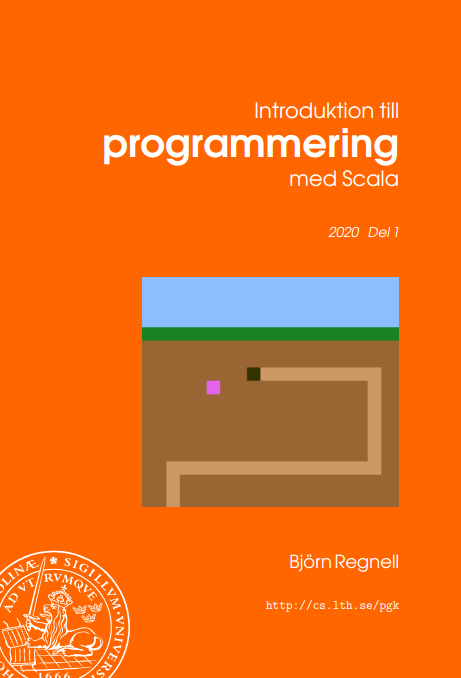
\includegraphics[width=0.35\textwidth]{../img/compendium-cover-part1-2020.png}%
~~~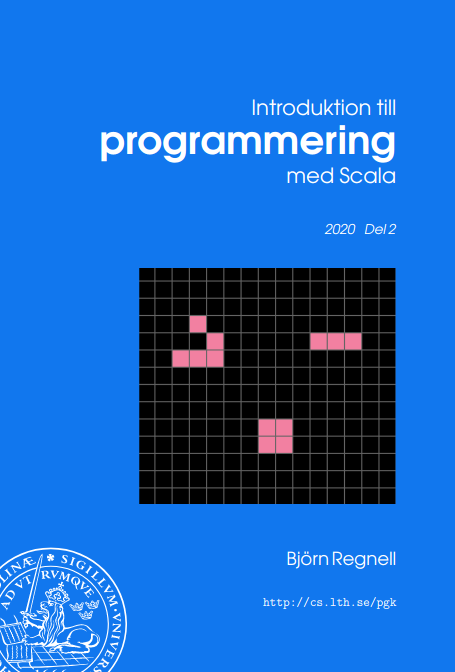
\includegraphics[width=0.348\textwidth]{../img/compendium-cover-part2-2020.png}
\begin{itemize}
\item \TODO \Emph{Kompendium}\\med övningar \& laborationer, \\trycks till självkostnad enl. beställning,\\se info bakom Canvas-väggen: \url{https://canvas.education.lu.se/courses/7756}
\item Föreläsningsbilder på kurshemsidan \\
 \url{http://cs.lth.se/pgk/}
\item Nätresurser enl. länkar i kursmaterialet

\end{itemize}
\end{minipage}
\hskip1em\begin{minipage}{0.35\textwidth}\SlideFontSize{8}{10}
Bra \Alert{bredvidläsning}:\\
-- för \Emph{nybörjare}:
\vskip0.2mm

\includegraphics[width=0.33\textwidth]{../img/lewisbook.jpg}\hskip4mm
%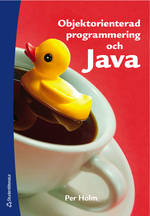
\includegraphics[width=0.33\textwidth]{../img/ankbok.jpg}

\noindent -- för de som \Emph{redan kan OO}:
\vskip0.7mm
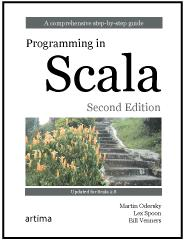
\includegraphics[width=0.45\textwidth]{../img/pinsbook.jpg}\hskip4mm
%
\includegraphics[width=0.47\textwidth]{../img/koffmanbook.jpg}
\end{minipage}
\end{SlideExtra}
\fi

\ifkompendium
\noindent Kompendiet är den huvudsakliga kurslitteraturen och definierar kursinnehållet. Föreläsningar, övningar och laborationer i kompendiet är kursens primära kunskapskällor, tillsammans med de öppna resurser på nätet som kompendiet hänvisar till. Kompendiet är öppen källkod och du välkomnas varmt att bidra!

Om du gärna vill ha en eller flera mer traditionella läroböcker som bredvidläsning rekommenderas följande:
\begin{itemize}[noitemsep, leftmargin=*]
\item För de som aldrig kodat, och vill läsa om kodning från grunden:
\begin{itemize}[nolistsep]
\item ''Introduction to Programming and Problem-Solving Using Scala'' Second Edition (2016), Mark C. Lewis, Lisa Lacher.  %{\href{https://www.crcpress.com/Introduction-to-Programming-and-Problem-Solving-Using-Scala-Second-Edition/Lewis-Lacher/p/book/9781498730952}{www.crcpress.com/Introduction-to-Programming-and-Problem-Solving-Using-Scala-Second-Edition/Lewis-Lacher/p/book/9781498730952}}

\item Lewis \& Lacher täcker stora delar av kursen, men innehåller även en del material som ingår i senare LTH-kurser. Ordningen är ganska annorlunda, men det går bra att läsa boken i en annan ordning än den är skriven.
% \item ''Objektorienterad programmering och Java'', Per Holm, Tredje upplagan (2007). \href{https://www.studentlitteratur.se/#6735}{www.studentlitteratur.se/\#6735}
\end{itemize}
\item För de som redan kodat en hel del i ett objektorienterat språk:
\begin{itemize}[nolistsep, noitemsep]
\item ''Programming in Scala'', Third Edition (2016), Martin Odersky, Lex Spoon, and Bill Venners.  %\\\href{http://www.artima.com/shop/programming_in_scala_3ed}{www.artima.com/shop/programming\_in\_scala\_3ed}
  \item Martin Odersky är upphovspersonen bakom Scala och denna välskrivna bok innehåller en komplett genomgång av Scala-språket med många exempel och tips. ''Third Edition'' täcker Scala version 2.12. Boken riktar sig till de som redan har kunskap om något objektorienterat språk, t.ex. Java. Det finns ett bra index som gör det lätt att anpassa din läsning efter kursens upplägg. Bokens ca 800 sidor innehåller mycket material som är på en mer avancerad nivå än denna kurs, men du kommer att ha nytta av innehållet i kommande kurser.
% \item ''Data Structures: Abstraction and Design Using Java, 3rd Edition'', Elliot B. Koffman, Paul A. T. Wolfgang. \\
% \href{http://eu.wiley.com/WileyCDA/WileyTitle/productCd-1119186528.html}{http://eu.wiley.com/WileyCDA/WileyTitle/productCd-1119186528.html}
\end{itemize}
\end{itemize}
Dessa läroböcker följer inte direkt kursens upplägg vad gäller omfång och progression och du får själv göra den nyttiga hemläxan att koppla  deras innehåll till det vi går igenom i kursens olika moduler.

\else


\begin{SlideExtra}{Bokpaketet}\SlideFontSmall
\begin{itemize}

\item \Emph{Kompendiet} finns i pdf för fri nedladdning enl. licensen CC-BY-SA, men det \Alert{rekommenderas starkt} att du även använder pappersversionen.

\item För de flesta funkar det mycket bättre att ha övningar och labbar \Alert{på papper} \Emph{bredvid skärmen}, när du ska tänka, koda och plugga!

\item \Emph{Snabbreferensen} finns också i pdf men du behöver ha en tryckt version eftersom det är \Alert{enda tillåtna hjälpmedlet} på skriftliga kontrollskrivningen och tentamen. \\ Säljs separat för 35kr på Datavetenskaps expedition.

\item Kompendiet och snabbreferens trycks här i E-huset och säljs av institutionen till \Emph{självkostnadspris} Se info i Canvas.

\end{itemize}
\end{SlideExtra}

\begin{SlideExtra}{Föreläsningsanteckningar}
\begin{itemize}
\item Föreläsningbilder uppdateras under kursens gång.
\item \url{http://cs.lth.se/pgk/foerelaesningar/}
\item Fram till mån kl 13 aktuell vecka är de bilder som ligger ute under pågående uppdatering sedan förra årets version.
\item Latex-koden för alla bilder finns här: \\
\href{https://github.com/lunduniversity/introprog/tree/master/slides}{github.com/lunduniversity/introprog/tree/master/slides}
\item Kom gärna med förslag på innehåll!
\end{itemize}
\end{SlideExtra}
\fi

\ifkompendium\else
\begin{SlideExtra}{Personal \CurrentYear}\SlideFontSmall
\begin{description}
\item [\bfseries Kursansvarig:] Prof. Björn Regnell, bjorn.regnell@cs.lth.se, E:2413
\item [\bfseries Handledare:]\Emph{teknologer:}\\
%2021
\TODO
%2020:
Anna	Johannesson,
Alexander	Sandström,
Evelina	Danielsson,
Emmanuel	Kring,
Emil	Wihlander,
Jos	Rosenqvist,
Jon	Swedberg,
Linnea	Allander,
Leo	Westerberg,
Madeleine	Berild,
Miro	Brodlova,
Maria	Svensson,
Nils	Ceberg,
Oskar	Berg,
Oliver	Persson,
Patrik	Fjellstedt,
Patrik	Gyllvin,
Paul	Wuilmart,
Rasmus	Beck,
Samer	Alkhodary,
Victor	Gunnnarsson,
Fritjof	Bengtsson
%2019:
% Alexander	Sandström, 
% Evelina	Danielsson, 
% Emil	Wihlander, 
% Hugo	Hildeman, 
% Henrik	Olsson, 
% Jos	Rosenqvist, 
% Jon	Swedberg, 
% Linnea	Allander, 
% Miro	Brodlova, 
% Oskar	Berg, 
% Oliver	Persson, 
% Rasmus	Beck, 
% Samer	Alkhodary
%2018:
% Emil Wihlander,
% Erik Präntare,
% Henrik Olsson,
% Ivar Henckel,
% Jonatan Nilsson,
% Jos Rosenqvist,
% Klara Broman,
% Linnea Bokelund,
% Ludvig Pärsson,
% Oliver Persson,
% Oskar Berg,
% Oskar Widmark,
% Samer Alkhodary,
% Stefan Jonsson,
% Victor Winberg
% \Emph{Koordinator}: \\
% %2017:
% Adjunkt Sandra Nilsson
%2017:
% Anders	Buhl,
% Erik	Grampp,
% Hampus	Weslien,
% Jakob	Hök,
% Johannes	Tykesson,
% Jonas	Danebjer,
% Jos	Rosenqvist,
% Ludvig	Pärsson,
% Måns	Magnusson,
% Martin	Jakobsson,
% Michael	Young,
% Oskar	Berg,
% Oskar	Widmark,
% Rasmus	Olsson,
% Roland	Holmberg,
% Stefan	Jonsson,
% Tobias	Bladh,
% Victor	Winberg
% % 2016: Doktorander MSc. Gustav Cedersjö, Tekn. Lic. Maj Stenmark \\
%2016:
%Anders Buhl,
%Anna Palmqvist Sjövall,
%Anton Andersson,
%Cecilia Lindskog,
%Emil Wihlander,
%Erik Bjäreholt,
%Erik Grampp,
%Filip Stjernström,
%Fredrik Danebjer,
%Henrik Olsson,
%Jakob Hök,
%Jonas Danebjer,
%Måns Magnusson,
%Oscar Sigurdsson,
%Oskar Berg,
%Oskar Widmark,
%Sebastian Hegardt,
%Stefan Jonsson,
%Tom Postema,
%Valthor Halldorsson
\item [\bfseries Kursadmin:]
Ulrika Templing, rum E:2179, Birger Swahn, rum E:2181 \\
Öppettider se här: 
\url{http://cs.lth.se/kontakt/expedition/} \\
\end{description}
\end{SlideExtra}
\fi


\begin{Slide}{Kursmoment --- varför?}\SlideFontTiny
\begin{itemize}

\item \Emph{Föreläsningar}: skapa översikt, ge struktur, förklara teori, svara på frågor, motivera varför.

\item \Emph{Övningar}: bearbeta teorin steg för steg, \Emph{grundövningar} för alla, \Emph{extraövningar} om du vill/behöver öva mer, \Emph{fördjupningsövningar} om du vill gå djupare; \Alert{förberedelse inför laborationerna}.

\item \Emph{Laborationer}: \Alert{obligatoriska}, sätta samman teorins delar i ett större program; lösningar redovisas för handledare; gk på alla för att få tenta.

\item \Emph{Resurstider}: få hjälp med övningar och laborationsförberedelser av handledare, fråga vad du vill.

\item \Emph{Samarbetsgrupper}: grupplärande genom samarbete, hjälpa varandra.

\item \Emph{Kontrollskrivning}: \Alert{obligatorisk}, diagnostisk, kamraträttad; kan ge samarbetsbonuspoäng till valfria tentan.

\item \Emph{Individuell projektuppgift}: \Alert{obligatorisk}, du visar att du kan skapa ett större program självständigt; redovisas för handledare.
\item \Emph{Muntligt prov}: \Alert{obligatoriskt}, ska klaras för godkänt på kursen; du visar att du har tillräcklig förståelse för kursens koncept för att klara nästa kurs. 

\item \Emph{Tentamen}: Valfri för överbetyg men alla uppmuntras att försöka; skriftlig, enda hjälpmedel: snabbreferensen.\url{http://cs.lth.se/pgk/quickref}
\end{itemize}
\end{Slide}

\ifkompendium\else
\begin{SlideExtra}{Detta är bara början... }
Exempel på efterföljande kurser som bygger vidare på denna:
\begin{itemize}
\item \Emph{Årskurs 1}
\begin{itemize}
\item Programmeringsteknik -- fördjupningskurs
\item Utvärdering av programvarusystem
\item Diskreta strukturer
\end{itemize}
\item \Alert{Årskurs 2}
\begin{itemize}
\item Objektorienterad modellering och design
\item Programvaruutveckling i grupp
\item Algoritmer, datastrukturer och komplexitet
\item Funktionsprogrammering
\end{itemize}
\end{itemize}
\end{SlideExtra}


% \begin{SlideExtra}{Registrering}
% \begin{itemize}
% \item Fyll i listan \Emph{REGISTRERING EDAA45} som skickas runt.

% \item Kryssa i kolumnen \Alert{ÅBEROPAR PLATS} om vill gå kursen\footnote{\scriptsize D1:a som redan gått motsvarande kurs? Uppsök studievägledningen}\footnote{\scriptsize D2:a eller äldre som redan påbörjad EDA016/EDA011/EDA017 el liknande? Övergångsregler: Alla labbar gk: tenta EDA011/017; annars kom och prata på rasten}

% \item Kryssa i kolumnen \Emph{KAN VARA KURSOMBUD} om du kan tänka dig att vara kursombud under kursens gång:
% \begin{itemize}
% \item Alla LTH-kurser ska utvärderas under kursens gång och efter kursens slut.
% \item Till det behövs kursombud -- minst \Alert{2 D-are} och \Alert{2 W-are}.
% \item Ni kommer att bli kontaktade av studierådet.
% \end{itemize}
% \item Om du ej ska gå kursen men vill bli indelad i schemagrupp skriv i kommentarskolumnen: \textit{''vill ha schemagrupp''}
% \end{itemize}
% \end{SlideExtra}

\fi


%%%
\ifkompendium\else

\begin{SlideExtra}{Förkunskaper}
\begin{itemize}
\item Förkunskaper $\neq$ Förmåga
\item Varken kompetens eller personliga egenskaper är statiska
\item ''Programmeringskompetens'' är inte \textit{en} enda enkel förmåga utan en komplex sammansättning av flera olika förmågor som \Emph{utvecklas} genom hela livet
\item Ett innovativt utvecklar\Alert{team} behöver många olika kompetenser för att vara framgångsrikt
\end{itemize}
\end{SlideExtra}


\SlideImg{Stor spridning i förkunskaper}{../img/survey-2020}

%%% AAAARGH -- version clash ? or something causing thins in Ubuntu 20.04 
%%%   but not in ubuntu 18.04:
%%%

    % ! Package pgfplots Error: Sorry, could not retrieve column 'år' from table '<i
    % nline_table>'. Please check spelling (or introduce name aliases)..

    % See the pgfplots package documentation for explanation.
    % Type  H <return>  for immediate help.
    %  ...                                              
                                                      
    % l.27 ...dplot table[x=år,y=nybörjare]{\dataSeq};
                                                      
    % !  ==> Fatal error occurred, no output PDF file produced!
    % Transcript written on lect-w01.log.

% \begin{SlideExtra}{Andelen D-are som vid kursstart aldrig kodat}
% \pgfplotstableread[row sep=\\,col sep=&]{
%     år & nybörjare\\
%     2015 & 19  \\
%     2016 & 32  \\
%     2017 & 38  \\
%     2018 & 31  \\
%     2019 & 30  \\
%     2020 & 20  \\
%     }\dataSeq

% \begin{minipage}{0.65\textwidth}
% \hspace*{-0.65cm}%
% \begin{tikzpicture}[scale=0.9, every node/.style={scale=0.9}]
%     \begin{axis}[
%             ybar,
%             bar width=1.0cm,
%             symbolic x coords={2015,2016,2017,2018,2019,2020},
%             xtick=data,
%             nodes near coords,
%             nodes near coords align={vertical},
%             legend style={at={(0.5,1)},anchor=south,legend columns=-1,draw=none},
%             ymin=0,ymax=45,
%             ylabel={\%},
%             xlabel={År},
%         ]
%         \addplot table[x=år,y=nybörjare]{\dataSeq};
%         %\legend{nybörjare}
%     \end{axis}
% \end{tikzpicture}
% \end{minipage}%
% \begin{minipage}{0.3\textwidth}
% \begin{itemize}\SlideFontTiny
% \item[] År: antal enkätsvar D
% \item[] 2015: 102 st
% \item[] 2016: 104 st
% \item[] 2017: 114 st
% \item[] 2018: 123 st
% \item[] 2019: 125 st 
% \item[] 2020: 137 st 
% \end{itemize}
% \end{minipage}%
% \end{SlideExtra}

\fi

\ifkompendium\else



%%%
% \begin{SlideExtra}{Förkunskapsenkät}
% \begin{itemize}
% \item Om du inte redan gjort det fyll i förkunskapsenkäten \Alert{snarast}:
% \url{http://cs.lth.se/pgk/introsurvey}
% \item Dina svar behandlas internt och all redovisad statistik anonymiseras.
% \item Enkäten ligger till grund för randomiserad gruppindelning i samarbetsgrupper, så att det blir en spridning av förkunskaper inom gruppen.
% \item Gruppindelning publiceras här, obs vänta på v1.0, Ctrl+F5: \\ \url{http://cs.lth.se/pgk/grupp}
% \item Ditt gruppnummer (t.ex. D1.7b) styr vilken schema grupp du tillhör (t.ex. D1.7), se \url{http://cs.lth.se/pgk/schema/timeedit/}
% \end{itemize}
% \end{SlideExtra}

\begin{SlideExtra}{Samarbetgrupper}\footnotesize
\begin{itemize}
\item Ni delas in i \Emph{samarbetsgrupper} om ca 5 personer baserat på förkunskapsenkäten, så att olika förkunskapsnivåer sammanförs
\item En av laborationerna (\code{snake}) i lp2 är en mer omfattande \Emph{grupplabb} och kommer att göras i din samarbetsgrupp. \\ \vspace{1em}
\item Kontrollskrivningen i halvtid kan ge \Emph{samarbetsbonus} (max 5p) som adderas till ordinarie tentans poäng (max 100p) med medelvärdet av gruppmedlemmarnas individuella kontrollskrivningspoäng
\scriptsize \parbox{7cm}{Bonus $b$ för varje person i en grupp med $n$ medlemmar med $p_i$ poäng vardera på kontrollskrivningen:}
 \hspace{5mm} $\displaystyle b = \sum\limits_{i=1}^n \frac{p_i}{n}$
\end{itemize}
\end{SlideExtra}



%%%
\begin{SlideExtra}{Varför studera i samarbetsgrupper?}

Huvudsyfte: \Emph{Bra lärande!}

\begin{itemize}
\item Pedagogisk forskning stödjer tesen att lärandet blir mer djupinriktat om det sker i utbyte med andra
\item Ett studiesammanhang med \Alert{höga ambitioner} och \Alert{respektfull gemenskap} gör att vi \Emph{når mycket längre}
\item Varför ska du som redan kan mycket aktivt dela med dig av dina kunskaper?
\begin{itemize}
\item Förstå bättre själv genom att förklara för andra
\item Träna din pedagogiska förmåga
\item Förbered dig för ditt kommande yrkesliv som mjukvaruutvecklare
\end{itemize}
\end{itemize}
\end{SlideExtra}

%%%

\begin{SlideExtra}{Samarbetskontrakt}
Gör ett skriftligt \href{https://github.com/lunduniversity/introprog/tree/master/study-groups}{\Emph{samarbetskontrakt}} med dessa och ev. andra punkter som ni också tycker bör ingå:
\begin{enumerate}
\item Återkommande mötestider per vecka
\item Kom i tid till gruppmöten
\item Var väl förberedd genom självstudier inför gruppmöten
\item Hjälp varandra att förstå, men ta inte över och lös allt
\item Ha ett respektfullt bemötande även om ni har olika åsikter
\item Inkludera alla i gemenskapen
\end{enumerate}

Diskutera hur ni ska uppfylla dessa innan alla skriver på. \\ Ta med samarbetskontraktet och visa för handledare på labb 1.

\vskip1em

\Alert{Om arbetet i samarbetsgruppen inte fungerar ska ni mejla kursansvarig och boka mötestid!}
\end{SlideExtra}

\begin{SlideExtra}{Dina frågor är viktiga!}
\begin{itemize}
\item Det finns bättre och sämre frågor vad gäller hur mycket man kan lära sig av svaret, men \Emph{all undran är en chans} att i dialog utbyta erfarenheter och lärande.
\item Den som frågar \Emph{vill veta} och berättar genom frågan något om nuvarande kunskapsläge.
\item Den som svarar får chansen att \Emph{reflektera} över vad som kan vara svårt och olika vägar till djupare förståelse.
\item I en hälsosam lärandemiljö är det \Emph{helt tryggt} att visa att man \Alert{ännu inte förstår}, att man gjort ''fel'', att man har mer att lära, etc.
\item Det är viktigt att \Emph{våga försöka} även om det blir \Alert{''fel''}:\\ \Alert{det är ju då man lär sig!}
\end{itemize}
\end{SlideExtra}

%%%
\begin{SlideExtra}{Plagiatregler}
\begin{itemize}
\item Läs dessa regler noga och diskutera i samarbetsgrupperna:

\begin{itemize}
\footnotesize
\item \url{http://cs.lth.se/utbildning/samarbete-eller-fusk/}
\item \href{http://cs.lth.se/utbildning/foereskrifter-angaaende-obligatoriska-moment/}{Föreskrifter angående obligatoriska moment}
\end{itemize}
\item Ni ska lära er genom \Emph{eget arbete} och genom  \Emph{bra samarbete}.
\item Samarbete gör att man lär sig bättre, men man lär sig \Alert{inte} av att kopiera andras lösningar.
\item \Alert{Plagiering är förbjuden} och kan medföra \Alert{disciplinärende och avstängning}.
\item Du får \Alert{INTE} lägga ut laborationslösningar öppet på \Emph{\code{github}} eller på annan plats där någon annan kan komma åt dem!
\end{itemize}

\end{SlideExtra}

\fi %%%%%%%%%%%%%%%%%%%%%%%%%%%%%%%%

%%%
\begin{Slide}{En typisk kursvecka}
\begin{enumerate}
\item Gå på \Emph{föreläsningar} på \Alert{måndag--tisdag}
\item \Alert{Jobba} \Emph{individuellt} med teori, övningar, labbförberedelser på  \Alert{måndag--torsdag}
\item \Alert{Träffas} i \Emph{samarbetsgruppen} och hjälp varandra att förstå mer och fördjupa lärandet, förslagsvis på återkommande tider varje vecka då alla i gruppen kan
\item Kom till \Emph{resurstiderna} och få hjälp och tips av handledare och kurskamrater på \Alert{onsdag--torsdag}
\item Genomför den obligatoriska \Emph{laborationen} på \Alert{fredag}
\end{enumerate}
Se detaljerna och undantagen i schemat: \href{http://cs.lth.se/pgk/schema}{cs.lth.se/pgk/schema}
\end{Slide}

\ifkompendium\else  %%%%%%%%%%%%%%%%%%%%%%%%%
%%%
\begin{SlideExtra}{Övningar}\SlideFontSmall
\begin{itemize}
  \item \Alert{Programmering lär man sig bäst genom att programmera...}

\item Genom övningarna bearbetar du teorins olika delar via egna \Emph{undersökningar} med \Alert{Scala REPL} som viktigaste verktyg.

\item Fokusera på att \Emph{förstå} vad som händer när du kör din kod. Om du bara rusar vidare utan reflektion lär du dig inte alls lika bra.

\item Till de flesta övningar finns facit. Titta inte på facit förrän du själv gjort ett försök. Det finns ofta många olika sätt att åstadkomma samma sak, och din lösningsvariant kan vara lika bra som den i facit -- använd REPL för att verifiera att din lösning fungerar. Diskutera med handledare om du är osäker på vad som är ok.

\item Skapa en miljö för \Emph{koncentration} och lärande \Emph{på djupet}. Stäng telefon, be kompisar i datorsalen att inte prata för högt, etc.
\end{itemize}
\end{SlideExtra}

\begin{SlideExtra}{Laborationer}\SlideFontSmall
\begin{itemize}
\item På laborationerna \Emph{sammanför} du veckans koncept till en \Emph{helhet} i ett större program och kollar att du \Alert{kan grunderna} inför kommande veckor.
\item Labbarna är \Emph{individuella} (utom en) och \Emph{obligatoriska}.

\item Gör \Emph{övningarna} och \Emph{labbförberedelserna} noga \Alert{innan} själva labben -- detta är ofta helt nödvändigt för att du ska hinna klart. Dina labbförberedelser kontrolleras av handledare under labben.

\item Är du \Emph{sjuk?} Anmäl det \Alert{före} labben till \url{bjorn.regnell@cs.lth.se}, \\ få hjälp på resurstid och redovisa på resurstid (eller labbtid, när handledaren har tid över)

\item Hinner du inte med hela labben? Se till att handledaren noterar \Alert{''kompletteras''}, och fortsätt på resurstid och ev. uppsamlingstider.

\item Läs noga kapitel noll ''\Alert{Anvisningar}'' i kompendiet!

\item Laborationstiderna är gruppindelade enligt \href{http://cs.lth.se/pgk/schema/}{schemat}. Du ska gå till den tid och den sal som motsvarar din grupp som visas i \href{http://cs.lth.se/pgk/schema/timeedit/}{TimeEdit}.\\
\item \Emph{Du hittar vilken grupp du tillhör i Canvas.}
% \Emph{Gruppindelning} blir ''klar'' senast i morgon tisdag kl 13.
% \\Nya versioner släpps här: \url{http://cs.lth.se/pgk/grupp}
% \\OBS! Rensa cachen (Ctrl+F5) och kolla versionsnummer.
\end{itemize}
\end{SlideExtra}


% %%%
% \begin{SlideExtra}{Resurstider}\SlideFontTiny
% \begin{itemize}
% \item På resurstiderna får du \Emph{hjälp}  med \Alert{övningar} och labb\Alert{förberedelser}.

% \item Kom till minst en resurstid per vecka, se \href{http://cs.lth.se/pgk/schema/timeedit}{Schema i TimeEdit}.

% %\item Handledare gör ibland \Emph{genomgångar} för alla under resurstiderna. Tipsa om handledare om vad du finner svårt!
% \item Du får i mån av plats gå på flera resurstider per vecka. Om det blir fullt i ett rum prioriteras schemagrupper:
% \end{itemize}
% \begin{table}[]
% \centering\SlideFontTiny
% \begin{tabular}{lllll}
% \Emph{Tid Lp1} & \Emph{Sal} & \Alert{Grupper med prio} \\
% \hline
% Ons 10-12 v1-7 & Alfa &  D1.09 \\
% Ons 10-12 v1-7 & Beta  &  D1.10 \\
% Ons 13-15 v1-7 & Alfa &  D1.07 \\
% Ons 13-15 v1-7 & Beta  &  D1.08 \\
% Ons 15-17 v1-7 & Alfa &  D1.03 \\
% Ons 15-17 v1-7 & Beta  &  D1.04 \\ \hline
% Tor 10-12 v1-7 & Alfa &  D1.01 \\
% Tor 10-12 v1-7 & Beta  &  D1.02 \\
% Tor 13-15 v1-7 & Alfa &  D1.11 \\
% Tor 13-15 v1-7 & Beta  &  D1.12 \\
% Tor 15-17 v1-7 & Alfa &  D1.05 \\
% Tor 15-17 v1-7 & Beta  &  D1.06 \\
% \end{tabular}
% \end{table}
% W-are tilldelas D-schemagrupp enl. samarbetsgruppindelningen.
% \end{SlideExtra}

\fi


% \ifkompendium\else
% \begin{SlideExtra}{Kursens virtuella maskin}
%   \begin{itemize}
%   \item Enklaste sättet att få igång kursens alla verktyg på din egen dator är att köra kursens virtuella maskin med hjälp av VirtualBox.
%   \item Installera virtualbox: \url{https://www.virtualbox.org/wiki/Downloads}
%   \item Ladda ner vm hemma (\Alert{inte} över eduroam för det är 5GB och tar en evighet): \url{http://cs.lth.se/pgk/vm}
%   \item Eller kopiera filerna från \Emph{USB-pinne} som går runt i salen. \\ 
%    Skicka vidare till nästa; lämna till Björn Regnell kl 15. \\
%     Om du inte hinner idag kan du kopiera på nästa gång.
%   \item Mer info finns i Appendix K i \href{http://cs.lth.se/pgk/compendium}{compendium.pdf} 
%   \end{itemize}
% \end{SlideExtra}
% \fi

% \ifkompendium\else
% \begin{SlideExtra}{På Rasten...}
% \begin{itemize}
%   \item Uppropslista fastställs
%   \item Ev. önskemål ang. gruppindelning pga speciella skäl
%   \item Bläddra i bredvidläsning
%   \item Beställning av \Alert{bokpaket} om du inte redan gjort det \url{http://cs.lth.se/pgk/bokpaket}
%   \item Fyll i \Alert{förkunskaper} om du inte redan gjort det \url{http://cs.lth.se/pgk/introsurvey}
%   \item ...
% \end{itemize}
% \end{SlideExtra}
% \fi

\ifkompendium\else
\begin{SlideExtra}{Ge din \textbf{hjärna} rätt förutsättningar för programmering}
  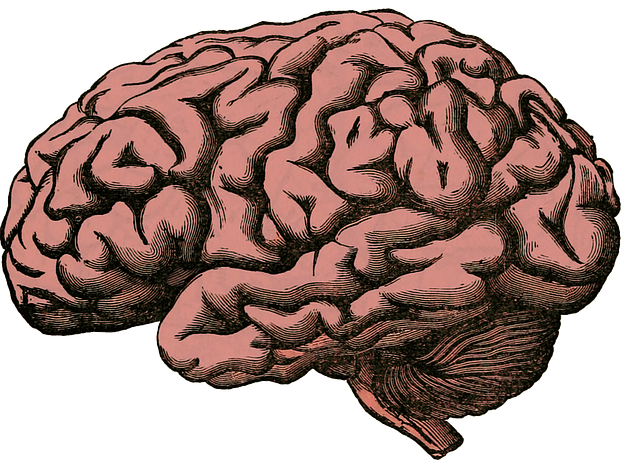
\includegraphics[height=0.9\textheight]{../img/brain.png}
\end{SlideExtra}
\fi
  